\documentclass[12pt, twoside]{book}
%\documentclass[12pt, oneside]{book}  % jednostranna tlac
\usepackage[a4paper,top=2.5cm,bottom=2.5cm,left=3.5cm,right=2cm]{geometry}
\usepackage[utf8]{inputenc}
\usepackage[T1]{fontenc}
\usepackage{graphicx}
\usepackage{url}
\usepackage[hidelinks,breaklinks]{hyperref}
%\usepackage[slovak]{babel} % vypnite pre prace v anglictine
\linespread{1.25} % hodnota 1.25 by mala zodpovedat 1.5 riadkovaniu

\usepackage{amssymb}
\usepackage[shortlabels]{enumitem}
\usepackage[utf8]{inputenc}
\usepackage{xstring}
\usepackage{mathtools}

\usepackage{tikz}
\usepackage{collcell}
\usepackage{relsize}
\usepackage{multirow}
\usepackage{comment}
\usepackage{pgfplots}

\pgfplotsset{width=12cm,compat=1.9}

%moje priklazy
\newtheorem{definition}{Definition}
\newtheorem{theorem}{Theorem}
\newtheorem{rovnica}{Equation}
\newtheorem{note}{Note}

\newcommand{\R}{\mathbb{R}}

% -------------------
% --- Definicia zakladnych pojmov
% --- Vyplnte podla vasho zadania
% -------------------
\def\mfrok{2021}
\def\mfnazov{Triangulation of implicit surface with singularities}
\def\mftyp{Master's thesis}
\def\mfautor{Bc. Kristína Korecová}
\def\mfskolitel{doc. RNDr. Pavel Chalmovianský, PhD. }

%ak mate konzultanta, odkomentujte aj jeho meno na titulnom liste
\def\mfkonzultant{tit. Meno Priezvisko, tit. }  

\def\mfmiesto{Bratislava, \mfrok}

% bioinformatici odkomentujú riadok s dvoma odbormi a iný program
\def\mfodbor{ Mathematics }
%\def\mfodbor{ Informatika a Biológia } 
\def\program{ Computer Graphics and Geometry }
%\def\program{ Bioinformatika }

% Ak je školiteľ z FMFI, uvádzate katedru školiteľa, zrejme by mala byť aj na zadaní z AIS2
% Ak máte externého školiteľa, uvádzajte Katedru informatiky 
\def\mfpracovisko{ Department of Algebra and Geometry }

\begin{document}     
\frontmatter


% -------------------
% --- Obalka ------
% -------------------
\thispagestyle{empty}

\begin{center}
\sc\large
Comenius University in Bratislava\\
Faculty of Mathematics, Physics and Informatics

\vfill

{\LARGE\mfnazov}\\
\mftyp
\end{center}

\vfill

{\sc\large 
\noindent \mfrok\\
\mfautor
}

\cleardoublepage
% --- koniec obalky ----

% -------------------
% --- Titulný list
% -------------------

\thispagestyle{empty}
\noindent

\begin{center}
\sc  
\large
Comenius University in Bratislava\\
Faculty of Mathematics, Physics and Informatics

\vfill

{\LARGE\mfnazov}\\
\mftyp
\end{center}

\vfill

\noindent
\begin{tabular}{ll}
Study Programme: & \program \\
Field of Study: & \mfodbor \\
Department: & \mfpracovisko \\
Supervisor: & \mfskolitel \\
% Konzultant: & \mfkonzultant \\
\end{tabular}

\vfill


\noindent \mfmiesto\\
\mfautor

\cleardoublepage
% --- Koniec titulnej strany


% -------------------
% --- Zadanie z AIS
% -------------------
% v tlačenej verzii s podpismi zainteresovaných osôb.
% v elektronickej verzii sa zverejňuje zadanie bez podpisov
% v pracach v aglictine anglicke aj slovenske zadanie

\newpage 
\thispagestyle{empty}
\hspace{-2cm}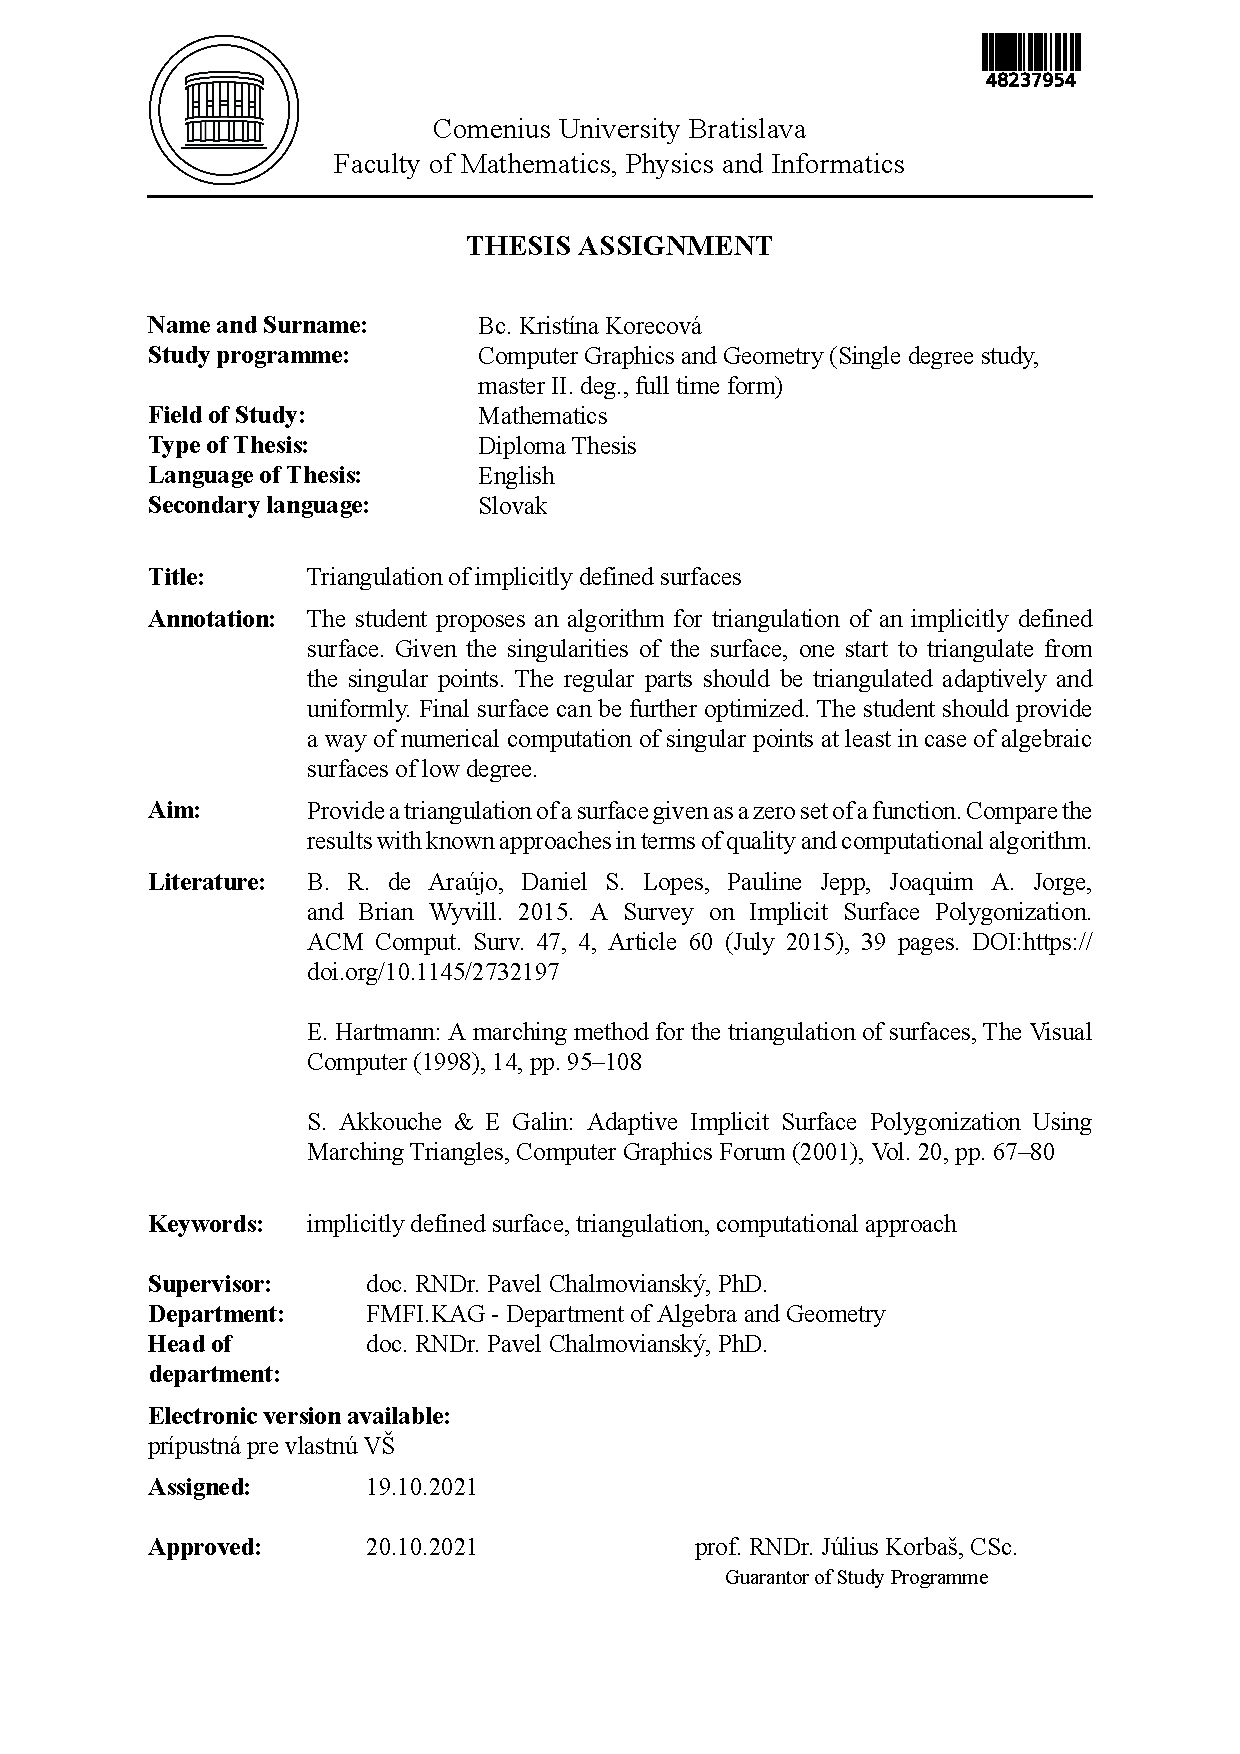
\includegraphics[page=1,width=1.1\textwidth]{images/zadanie-en}
\hspace{-2cm}\includegraphics[page=2,width=1.1\textwidth]{images/zadanie-en}

% --- Koniec zadania

\frontmatter

% -------------------
%   Poďakovanie - nepovinné
% -------------------
\setcounter{page}{3}
\newpage 
~

\vfill
{\bf Acknowledgements:} TODO Acknowledgements

% --- Koniec poďakovania

% -------------------
%   Abstrakt - Slovensky
% -------------------
\newpage 
\section*{Abstrakt}

Implicitne zadané plochy sú plochy, ktoré sú definované ako nulová hladina
funkcie troch premenných. Triangulácia plochy je častý spôsob digitálnej reprezentácie
plochy.
Pre množstvo algoritmov, ktoré vytvárajú aproximáciu trojuholníkovým meshom,
vznikajú problémy ak plocha obsahuje singularity -- body v ktorých je gradient funkcie
nulový vektor.
Niektoré algoritmy, ako napríklad Marching Cubes \cite{lorensen1987marching},
jednoducho ignorujú singulárne body, čo vedie k nekorektnej aproximácií plochy.
V tejto práci vytvárame algoritmus na trianguláciu plôch zadaných implicitne
obsahujúcich niktoré typy singuarít, pričom sa zameriavame na korektnosť
triangulácie a kvalitu meshu.
Rozširujeme algoritmus implementovaný v bakalárskej práci \cite{korecova2021triangulation}
založený na algoritme Marching Triangles \cite{hilton1996marching}
aby umožnil trianguláciu implicitne zadaných plôch obsahujúcich 
ADE singularity a krivkové singularity na prieniku dvoch regulárnych plôch.
Navyše navrhujeme prístup na vytvorenie triangulácie adaptívnej na 
lokálnu krivosť plochy. Nakoniec reimplemenutujeme algoritmus 
\cite{korecova2021triangulation} pre zrýchlenie času behu algoritmu.
\paragraph*{Kľúčové slová:} implicitne definovaná plocha, triangulácia, výpočtový prístup

% --- Koniec Abstrakt - Slovensky


% -------------------
% --- Abstrakt - Anglicky 
% -------------------
\newpage 
\section*{Abstract}
Implicit surfaces are surfaces defined as a zero set of a function.
Triangulation of the surface is a common way of the digital surface
representation.
For most algorithm constructing the approximation by the triangular mesh
a problem arises if the surface contains singularities -- the points at which 
the gradient of the defining function vanishes.
Some algorithms, such as the Marching Cubes \cite{lorensen1987marching},
simply ignore the singular points, which results in the incorrect approximation
of the surface.
In this thesis, we create an algorithm for triangulation of 
the surfaces with certain types of singularities, while focusing on the
correctness of the triangulation and the quality of a mesh.
We are extending the algorithm implemented in the bachelor's thesis 
\cite{korecova2021triangulation}
based on the Marching Triangles \cite{hilton1996marching} to allow 
triangulation of the implicit surfaces containg ADE singularities
and curve singularities on the intersection of two regular surfaces.
Moreover, we propose an approach to create a triangulation adaptive 
to the local curvature of a surface. Lastly, we reimplement the 
algorithm \cite{korecova2021triangulation} to speed up its runtime.
\paragraph*{Keywords:} implicitly defined surface, triangulation, computational approach

% --- Koniec Abstrakt - Anglicky

% -------------------
% --- Predhovor - v informatike sa zvacsa nepouziva
% -------------------
%\newpage 
%\thispagestyle{empty}
%
%\huge{Predhovor}
%\normalsize
%\newline
%Predhovor je všeobecná informácia o práci, obsahuje hlavnú charakteristiku práce 
%a okolnosti jej vzniku. Autor zdôvodní výber témy, stručne informuje o cieľoch 
%a význame práce, spomenie domáci a zahraničný kontext, komu je práca určená, 
%použité metódy, stav poznania; autor stručne charakterizuje svoj prístup a svoje 
%hľadisko. 
%
% --- Koniec Predhovor


% -------------------
% --- Obsah
% -------------------

\newpage 

\tableofcontents

% ---  Koniec Obsahu

% -------------------
% --- Zoznamy tabuliek, obrázkov - nepovinne
% -------------------

\newpage 

\listoffigures
\listoftables

% ---  Koniec Zoznamov

\mainmatter

%názvy kapitol

\input uvod.tex 

\input kapitola1.tex

\input kapitola2.tex

\input kapitola3.tex

\input kapitola4.tex

\input zaver.tex

% -------------------
% --- Bibliografia
% -------------------


\newpage	

\backmatter

\thispagestyle{empty}
\clearpage

\bibliographystyle{plain}
\bibliography{literatura} 

%Prípadne môžete napísať literatúru priamo tu
%\begin{thebibliography}{5}
 
%\bibitem{br1} MOLINA H. G. - ULLMAN J. D. - WIDOM J., 2002, Database Systems, Upper Saddle River : Prentice-Hall, 2002, 1119 s., Pearson International edition, 0-13-098043-9

%\bibitem{br2} MOLINA H. G. - ULLMAN J. D. - WIDOM J., 2000 , Databasse System implementation, New Jersey : Prentice-Hall, 2000, 653s., ???

%\bibitem{br3} ULLMAN J. D. - WIDOM J., 1997, A First Course in Database Systems, New Jersey : Prentice-Hall, 1997, 470s., 

%\bibitem{br4} PREFUSE, 2007, The Prefuse visualization toolkit,  [online] Dostupné na internete: <http://prefuse.org/>

%\bibitem{br5} PREFUSE Forum, Sourceforge - Prefuse Forum,  [online] Dostupné na internete: <http://sourceforge.net/projects/prefuse/>

%\end{thebibliography}

%---koniec Referencii

% -------------------
%--- Prilohy---
% -------------------

%Nepovinná časť prílohy obsahuje materiály, ktoré neboli zaradené priamo  do textu. Každá príloha sa začína na novej strane.
%Zoznam príloh je súčasťou obsahu.
%
\input appendixA.tex

%\input appendixB.tex

\end{document}






